\section{Versuchsdurchführung} 
\label{sec:versuchdurchführung}
Die Durchführung des Versuchs lässt sich auf auf 2 Themen reduzieren. Den Aufbau %\ref{sec:Aufbau}
und die Durchführung %\ref{sec:Durchführung}
selbst. Im Aufbau wird beschrieben, 
welcher Werkstoff mit welchen geometrischen Eigenschaften benutzt wird und die dazugehörigen Messgeräte werden diskutiert. Dazu kommt eine Auflistung der Geräte, die Strom erzeugen oder 
auswerten können. Im Teil der Durchführung %\ref{sec:Durchführung}
wird eine Überischt der einzelnen Schritte geschaffen und jeweils diskutiert.


\subsection{Aufbau und Materialien}
\label{sec:Aufbau}
Der Werkstoff des Versuchses war primär Kupfer. Zur Verfügung standen ein Kupferdraht und ein Kupferblech. Der Draht diente lediglich der Bestimmung des Wiederstadnes während 
das Blech später zur Hall-Sonde funktioniert wurde. 
Das Magnetische Feld wurde durch einen in Reihe geschalteten Elektromagneten erzeugt. Zur Analytischen Auswertung diente ein Multimeter und ein Teslameter.\\

\vspace{1cm}
\begin{minipage}{0.5\textwidth}
\centering
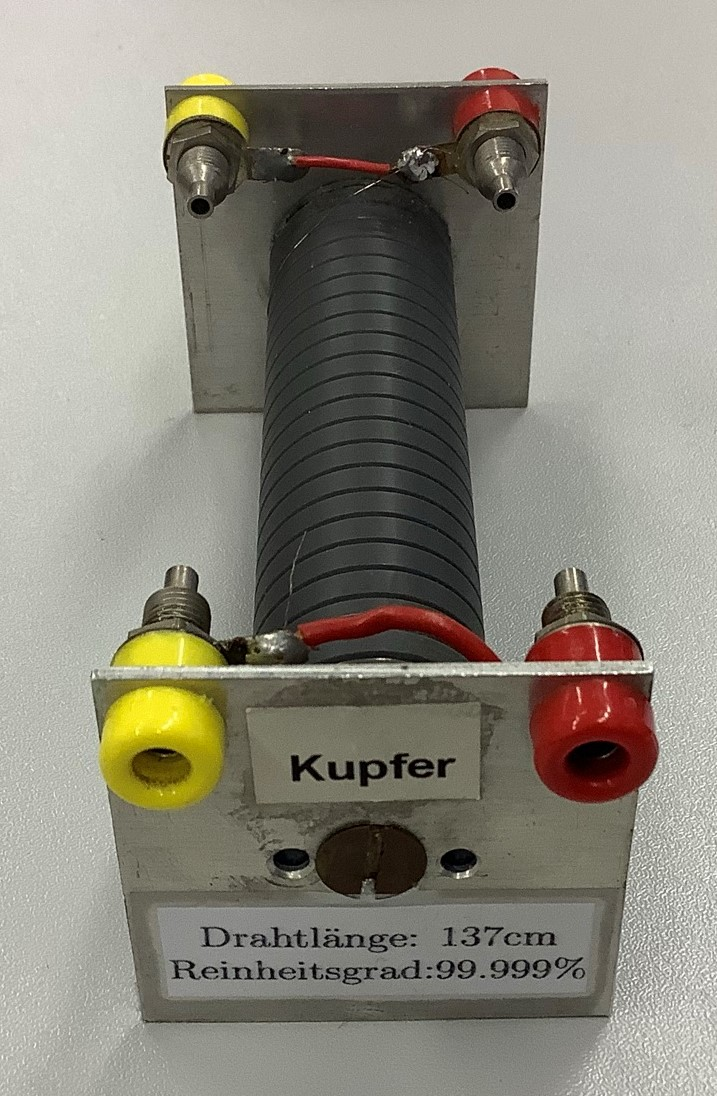
\includegraphics[height=5cm]{bilder/Kupferdraht.png}
\captionof{figure}{Kupferdraht \\ zur Bestimmung  des Wiederstadnes }
\label{fig:Kupferdraht}
\end{minipage}
\hfill
\begin{minipage}{0.49\textwidth} 
\centering
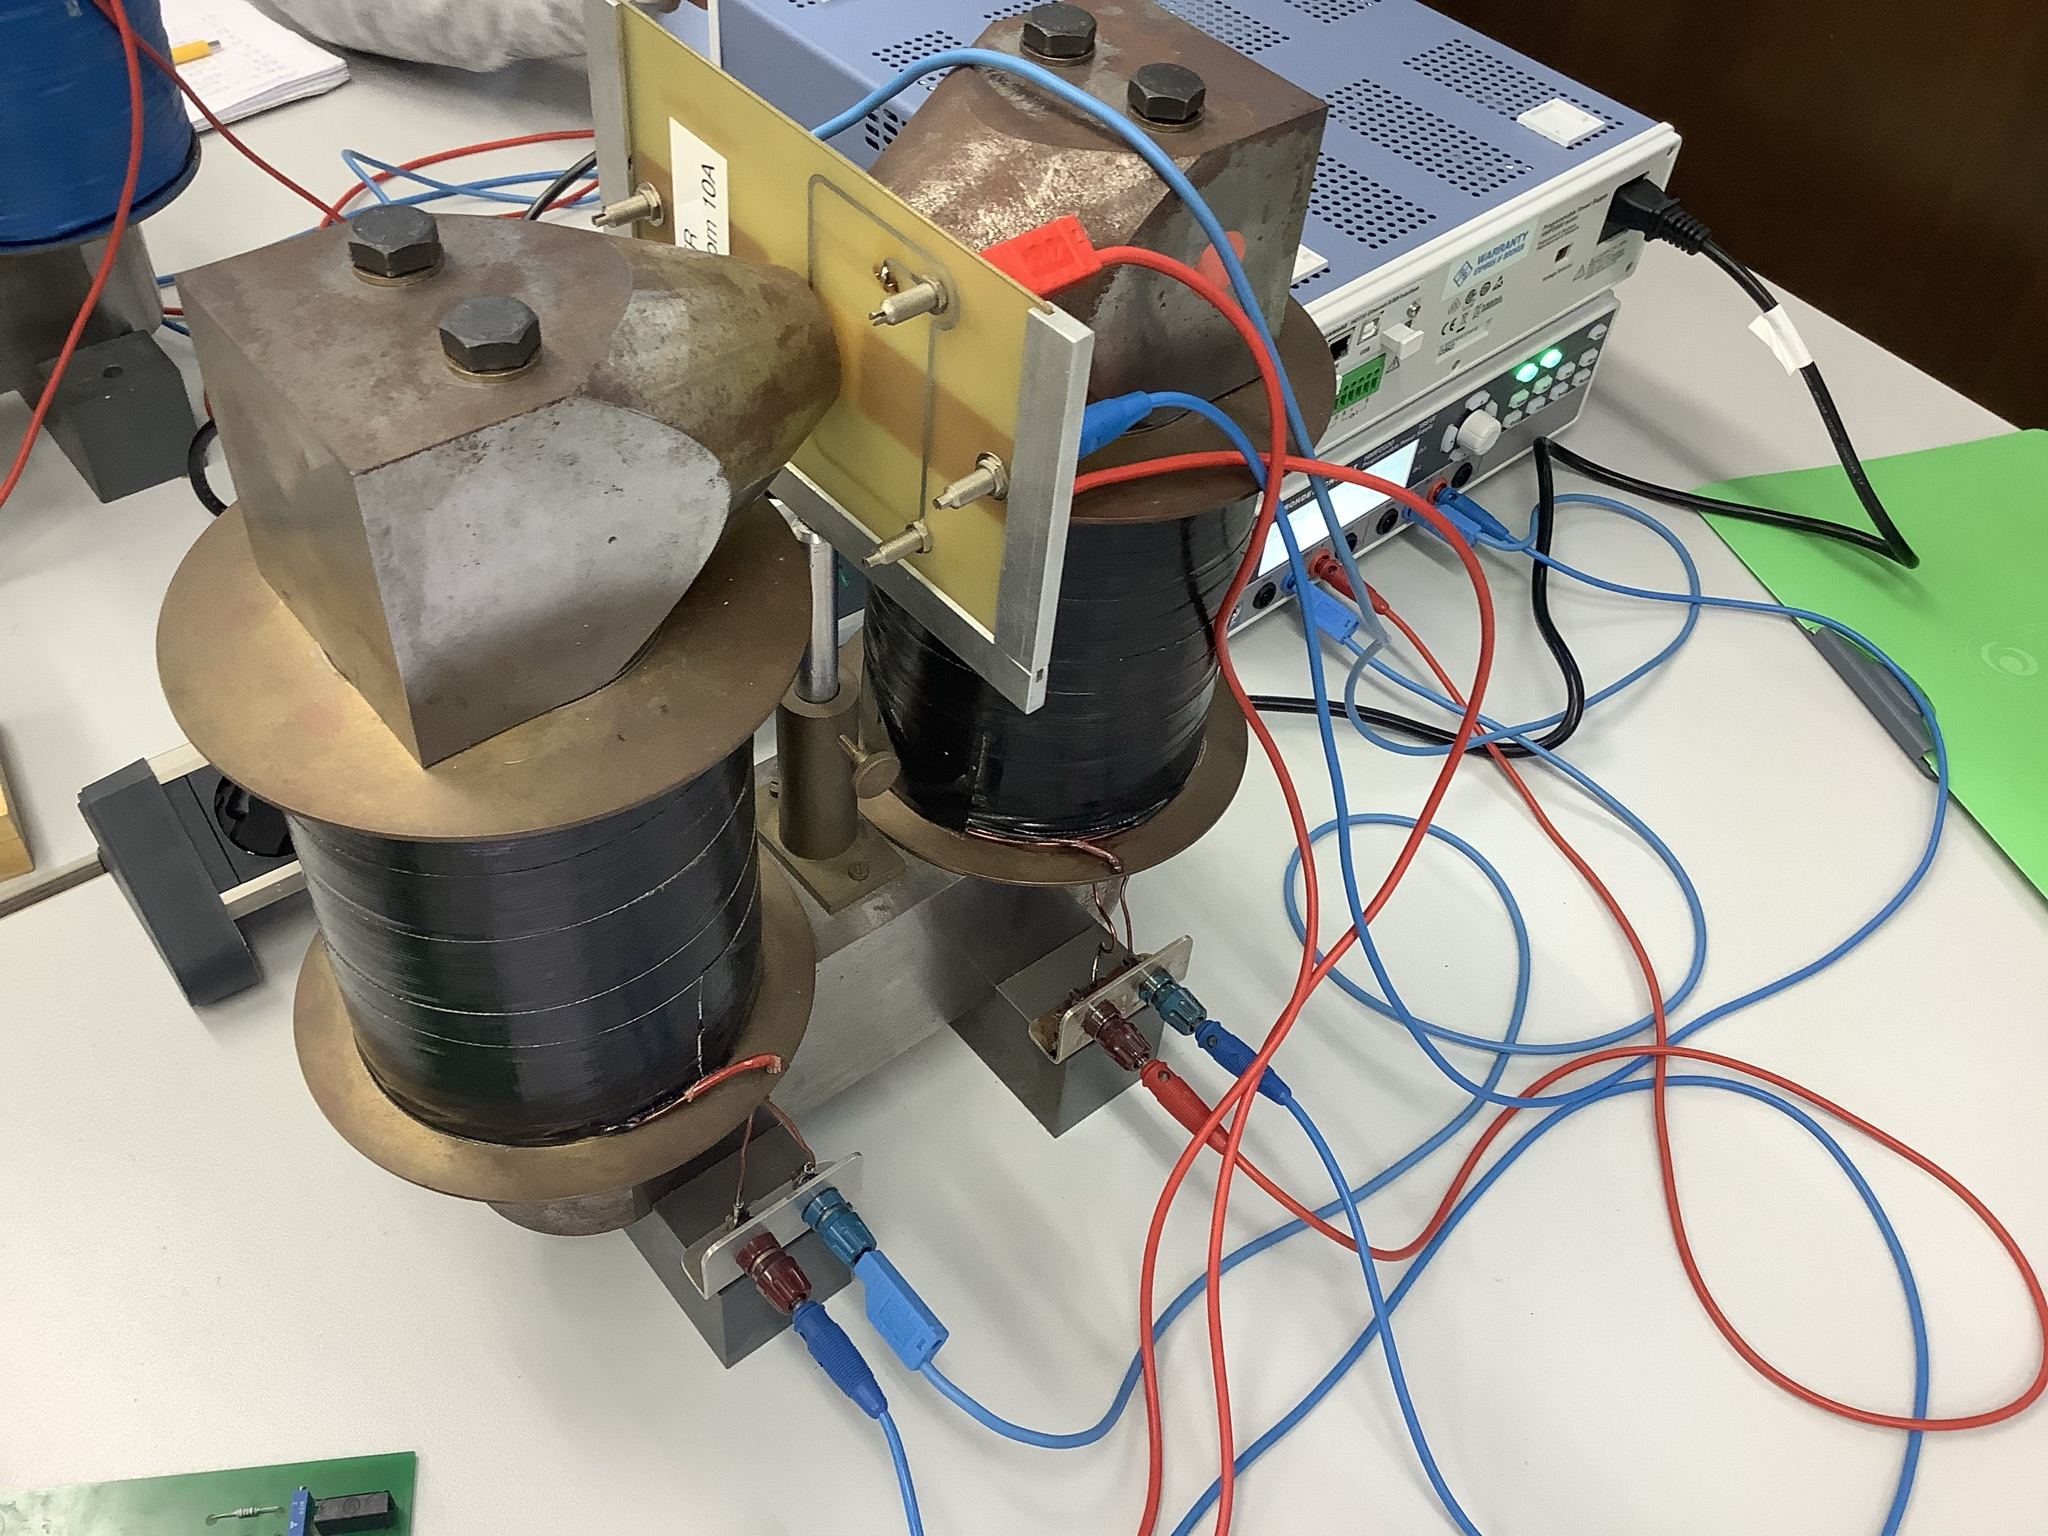
\includegraphics[height=5cm]{bilder/Magnet.png}
\captionof{figure}{Magnet\\ mit eingesetzem Kupferblech}
\label{fig:Magnet}
\end{minipage}

\subsection{Versuchsanordnung des Kupferblechs}
\label{sec:Blech}
%VIELE verweise zur Theorie
Das Blech wird an den äußeren Seiten mit einer Spannung belegt, mit dem Ziel die frei beweglichen Leitungselektronen auf eine Geschwindigkeit parallel zum 
Blech zu bringen. Diese Spannung bewirkt einen Strom $\text{\textbf{I}}_q$. Das Magnetische Feld würde, entsprechend der Bedingung aus der Lorentz Kraft \eqref{eqn:lorentz},
senkrecht auf dem Blech stehen. Um die sogenannte \textbf{Hall-Spannug} $U_H$ an den zwei langen Seiten des Bleches zu messen, wird dort ein Stromkreis
mit einem eingeschlossenen digitalen Voltmeter angelegt. Das Blech ist mit einer Dicke $d$ und einer Breite $b$ gegeben.

\begin{figure}
     \centering
     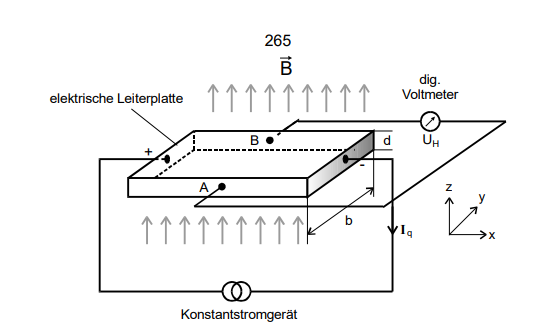
\includegraphics[width=\textwidth]{bilder/versuchsanordnung.png}
     \caption{Kupferblech mit entsprechnder Anordnung der Messgeräte}
     \cite[9]{V311.pdf}
     \label{fig:kupferblech}
\end{figure}

\subsection{Versuchsdurchführung}
Begonnen wird mit der Feststellung des Wiederstandes von Kupfer. An dem Draht lässt sich durch ein Messgerät eine Spannung anlegen und durch das Ohmsche Gesetz
den Wiederstand bestimmmen. \\ \flushleft

Nun wird sich dem Blech zugewandt, welches nachher in das Magnetfeld gelegt werden soll, und somit eine \textbf{Hall-Spannung} erfährt.
Wichtig ist, dass das Blech aus dem gleichen Material ist wie der Draht auch. In diesem Fall Kupfer. Die Dicke $d$ stellt eine siginifikante Größe da, wird also genau gemessen.\\ \flushleft


Anschließend wird die Hytseresekurve % eventuell ref 
des Magnetfeldes bestimmmt um eventuelle Unsicherheiten im späteren Verlauf der Auswertung auszuschlißen. Um nämlich Aufschluss über das 
tatsächlihce Verhältnis von Strom zu Feldstärke zu bekommen, muss man eben diese Kurve kennnen, mitsamt  Remanenzwert. % \ref{} --> Theorire eventuell?
                                                                                                                       % \ref{} --> Section der auswertung
Die Messung verläuft mithilfe eines Gerätes, dass die magnetische Feldstärke messen kann, hier wurde ein Teslameter verwendet.   
Wichtig ist hier, sowohl die Veränderung bei steigendem, sowie abfallendem Strom auszuwerten.  \\ \flushleft

Im nun bekannten Magnetfeld wird jetzt das Blech senkrecht zum Feld eingestellt und der Strom $\text{I}_q$ in möglichsts kleinen Schritten, bei Null beginnend, erhöht. 
Am Multimeter lässt sich nun eine Spannung ablesen, die wir vohrer als \textbf{Hall-Spannung} $\text{U}_H$  identifiziert haben. In Aussicht auf andere Ergebnise 
wurde die Ausrichtung des Pols von $\text{I}_q$ geändert und die Spannung nocheinmal analog gemessen. Die Ergebnisse liefern Daten für das Verhältnis zwischen 
der \textbf{Hall-Spannung} $\text{U}_H$ und der an dem Blech aneglegten Strom $\text{I}_q$ bei konstantem Magnetfeld mit $5$m$\si{\tesla}$.\\ \flushleft

Der Aufbau bleibt im letzten Schritt bestehen, jedoch wird nun $\text{I}_B$ und somit das Magnetfeld zum variablen Paramter. Der Strom durch das Blech auf einen 
konstanten Wert von $5\si{\ampere}$ gestellt. Es folgen Messungen für beide Polrichtungen des variablen Stroms $\text{I}_B$ welche wieder zur Spannung $\text{U}_H$ führen.
                                                                                                                    
                                                      